%% The following is a directive for TeXShop to indicate the main file
%%!TEX root = diss.tex
\chapter{Random walk models with general constraints}

%================================
\section{Introduction}
%================================
We will push the operator notation further to see what kinds of random walk models we can handle. Some of the models have more general step sets while others are set in more complicated regions. For example, Definition 1.1 of \cite{mishna2009classifying} has a functional equation for the non-interacting random walks on the quarter plane, which is valid for models with $\mc S$ containing negative coordinates of size at most $\um 1$. Similarly, \cite{kauers2014walks} covers walks in the quarter plane with multiple copies of small steps. We start with the following definition for a random walk model in $\ze^d$.
\begin{definition} Let $\mc{D}_0 \subseteq \mc{D}$ be regions in $\ze^d$ and $\mc S$ be a set of $d$-tuples in $\ze^d$. A triple $\mc{M} = (\mc{S}, \mc{D},\mc{D}_0)$ is a random walk model $\mc{M}$ with steps $\mc{S}$, living in the region $\mc{D}$ and interacting with region $\mc{D}_0$. We may impose a starting location later on.
\end{definition}
In other words, we are given a set of steps $\mc{S}$ and a starting location in $\mc{D}$. Then we want to evolve the random walks restricted to the region $\mc{D}$. We also have some special locations $\mc{D}_0$ within $\mc{D}$, and we wish to count the interactions of the random walks with points in this region. The interactions may be further specified later on.

\begin{figure}[H]
    \centering
    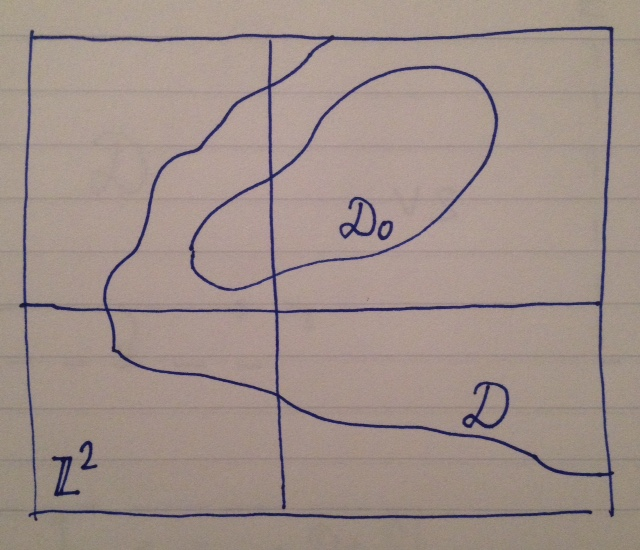
\includegraphics[scale = 0.5]{image1}
    \caption{General regions in $\ze^2$}
\end{figure}

For example, we may consider a semi-infinite strip on the plane as in \cite{brak2005directed}, \cite{wong2014confining} and \cite{owczarek2012enumeration}. In \cite{niederhausen2005note} the author considers random walks in an octant with interactions with the diagonal.

\begin{definition} Let $\mc{M}$ be a random walk model and $Q$ its associated generating function counting length with $t$, ending locations with $\row xd$, and interactions with $\mc{D}_0$ with some multi-index variable $a$. We write
\begin{align}
	Q = Q(\row xd,a;t) = \sum_{k=0}^{\infty} q_k(\row xd, a)t^k
\end{align}
where $q_k$ are Laurent poynomials in the $x$ and $a$ variables. 
\end{definition}
\begin{definition} Suppose that $\Gamma$ is an operator involving the $x$ and $a$ variables but not $t$. We shall apply $D$ on power series $F = \sum_{k=0}^\infty f_k t^k$ in the following linearized way
\begin{align}
	\Gamma F = \sum_{k=0}^\infty \Gamma (f_k) t^k
\end{align}
to avoid problems in expanding $F$ in Laurent series in some of the $x$ variables.
\end{definition}

\begin{definition} Let $\mc{M}$ be a given model. We will denote with $S$ the Laurent polynomial (or series) keeping inventory of the steps $\mc{S}$. Let $K = 1-tS$ be the Kernel of $\mc{M}$. Let $E$ be an operator that eliminates monomials $x_{[d]}^P$ when $P$ is not in $\mc{D}$. Let $L$ be an operator that marks (or labels) monomials $x_{[d]}^P$ for $P \in \mc{D}_0$ in a specified way in the model. Note that $L$ is invertible with inverse $L^{\um 1}$ that is given by marking with $1/a$ instead.
\end{definition}

This operator notation allows us to write down functional equations for $Q$ really quickly.
\begin{theorem} Let $\mc{M}$ be a random walk model and $Q$ its associated generating function with an initial term $q_0 = q$. Then $Q$ satisfies the following functional equations
\begin{align}
	(1-tLES)Q &= q\\
	(L^{\um 1}-tES)Q &= L^{\um 1}(q) = \alpha
\end{align}
\end{theorem}
\begin{proof} The second functional equation is obtained by applying $L^{\um 1}$ on the first one, so it only remains to show that the first functional equation holds. We do this via iteration. We start with $Q$ and multiply it with $tS$. This gives $tSQ$ or an enumeration of all walks extended by a single step. Here the power of $t$ is raised by one to keep track of this extension. Then we apply $E$ to this result to eliminate all random walks that venture outside of the region $\mc{D}$. Finally, we mark those walks that have arrived at locations in $\mc{D}_0$ by applying $L$ to $E(tSQ)$. The resulting expression is almost $Q$, but one term is missing - namely, $q_0 = q$. That is, we have transformed $Q$ to itself in a nontrivial way and we have the equation
\begin{align}
	Q = q + LE(tSQ) = q + tLE(SQ)\,,
\end{align}
and to complete the proof, we rewrite the equation to the form at the start of the theorem.
\end{proof}

\begin{example} Also, we can consider a different approach where instead of removing walks that venture outside of $\mc{D}$ we just mark them with some variable $z$ for later deletion. Suppose that we are given some model $\mc{M}$ and we want to frame the analysis in this new way. We have a new random walk model $\wcal{M}$ with $\wcal{D} = \ze^d$ and $\wcal{D}_0 = \mc{D}_0 \cup \mc{D}^c$, where we mark monomials in $\mc{D}^c$ with $z$ and those in $\mc{D}_0$ in the same way as in model $\mc{M}$. Here $\widetilde{E}$ is the identity operator since we do not remove any walks. We have the functional equations
\begin{align}
(1-t\widetilde{L} S)\widetilde Q &= q\,,\\
(\widetilde{L}^{\um 1}-tS) Q &= \widetilde{\alpha}\,.
\end{align}
It is not clear how one would proceed and if this would be a better way to handle the problem. The upside is that the operators are invertible, but the downside is that we now have more extracted terms in the functional equation, since the random walks can now go anywhere.
\end{example}

Next, we can talk about some of the abstract properties of the operators $L$ and $E$. The operator $E$ has the eigenvalues 1 or 0 for monomials $x_{[d]}^P$ where $P \in \mc{D}$ or $P \in \mc{D}^c$ respectively. The latter characterizes the monomials contained in $\ker E$. Similarly, $L$ has eigenvalues 1 for when $P \in \mc{D}_0^c$, and the marking monomial $a$ for when $P\in \mc{D}_0$. Here $a$ will vary from point to point. Also, $L^{\um 1}$ will have the reciprocal eigenvalues of $L$.

The task for the rest of the chapter is to come up with representations for the operators involved. In general, this should not be an easy task because if we could express arbitrary operators $L$ and $E$ with a small number of coefficient extractions, we would also be able to use this scheme to compress data without loss, and this is impossible in general.


%================================
\section{Marking Operators}
%================================
The example in the previous section shows that we can talk about marking operators on their own without considering operators $E$. Alternatively, the operators $E$ are just marking operators that apply a label $a = 0$. Therefore, we can combine the discussions for operators $L$ and $E$. Whenever invertibility is concerned, the discussion will apply to operators $L$ only. Suppose that we wish to mark points $p \in P\subseteq \ze^d$ with labels $a_p$ via an operator $\Gamma_P$. It can be written as
\begin{align}
	\Gamma_P = 1 + \sum_{p\in P}(a_p-1) \ext{x_{[d]}^p}\,.
\end{align}
The form $a_p-1$ follows from the fact that we have the original term and we need to remove it before marking with $a_p$. In the case where we mark points for deletion, $P = {\mc{D}}^c$ and $a_p = a$. In the models we have investigated so far we saw that we do not really need the whole operator but just some terms near the boundaries.
\begin{example} If we consider random walks with small steps on the half-line in one dimension, we have the operator
\begin{align}
	E = 1 - \sum_{n=1}^\infty \ext{\ol{x}_1^n}\,,
\end{align}
but since we only have small steps, there are no walks that go past $\ol{x}_1$ in the negative direction. Therefore, we can use the operator $E' = 1- \ext{\ol{x}_1}$ to the same effect instead. Although the operators are different in form, they are essentially the same with regards to the problem at hand. We will say they are model-equivalent.
\end{example}
To make things easier, we may think of the random walk models as living completely within the sumset $\mc{S}+\mc{D}$ of points that are combinations of points in $\mc{D}$ and steps $\mc{S}$. This is how far walks from the model can reach from within $\mc{D}$ by taking a single step.
\begin{definition} Given sets $A$ and $B$, we let their sumset be defined as
\begin{align}
	A+ B = \{a+b\,|\,a\in A,\, b\in B\}\,.
\end{align}
\end{definition}
\begin{definition} Given a random walk model $\mc{M}$ with domain $\mc{D}$ and step set $\mc{S}$, define the reach of model $\mc{M}$ to be the sumset $\mc{D}+\mc{S}$.
\end{definition}
With this in mind, we can define a notion of equivalence for operators.
\begin{definition} Let $\mc{M}$ be a random walk model in $\ze^d$ and let $\Gamma$ and $\Gamma'$ be two operators acting on $\ze^d$. Then $\Gamma \equiv_{\mc{M}} \Gamma'$ if and only if $\Gamma$ and $\Gamma'$ act the same way on monomials from the reach of $\mc{M}$. That is, we call these operators model-equivalent if and only if $\Gamma  x^P = \Gamma' x^P$ for all $P\in \mc{D}+\mc{S}$.
\end{definition}
In the preceding example $E\equiv E'$ since they act the same way on monomials from the reach of $\mc{M}$, that is, monomials $x_1^n$ for $n\ge \um 1$. Similarly, in the two-dimensional problem we have an equivalence between the operator $E$ and the operator $E' = (1-\ext{\ol{x}_1})(1-\ext{\ol{x}_2})$.
\begin{align}
	\Gamma = 1 + (a-1)\sum_{k=1}^{\infty} \ext{\ol{x}^k} = 1 + (a-1)\sum_{k=1}^{n} \ext{\ol{x}^k}
\end{align}
When the boundary of $\mc{D}$ is complicated, we may not find nice model-equivalent operators, but there are some cases where we can say something. In the usual problem we have an operator $E$ with infinitely many terms, but instead, we find that there is a model-equivalent operator $E'$ that is only comprised of finitely many terms. We will investigate which operators have finite equivalent operators.
\begin{definition} Given a model $\mc{M}$, a coefficient extraction operator $\Gamma$ in the variables $\row xd$ is of finite type if it is equivalent to an operator $\Gamma'$ that only has finitely many coefficient extraction terms. That is,
\begin{align}
	\Gamma \equiv_{\mc M} \Gamma' = \sum_{\substack{I\subseteq [d]\\ J \subseteq \ze^d}}a_{I,J} \ext{x_I^J}
\end{align}
where each $|J| < \infty$. We will say that $\Gamma'$ is of infinite type if it is not of finite type.
\end{definition}
For most purposes we will not distinguish between $\Gamma$ and $\Gamma'$. A natural question is to consider which models $\mc{M}$ lead to operators of finite type. This very much depends on the region $\mc D$ and the nature of the marking of region $\mc D_0$. We have some cases where it is easy to say.

\begin{lemma} Let $\mc D$ be a $d$-dimensional box in $\ze^d$ and $|\mc S| < \infty$. Then the operator $\Gamma = LE$ is of finite type.
\end{lemma}
\begin{proof} The operator $L$ is finite since it only needs to mark finitely many points. We can find $E$ explicitly. Let the box have $x_k$ coordinates $[a_k,b_k]$. Suppose that the steps in $\mc S$ have $x_k$ coordinates of absolute size at most $n_k$. If $n_k = 0$, the walks do not change their $x_k$ coordinate and the walks do not venture past the boundaries in that coordinate. When $n_k > 0$ we need to remove all monomials $x^P$ with $P_k \in [a_k-n_k,a_k-1]\cup [b_k+1,b_k+n_k]$. 

\begin{figure}[H]
    \centering
    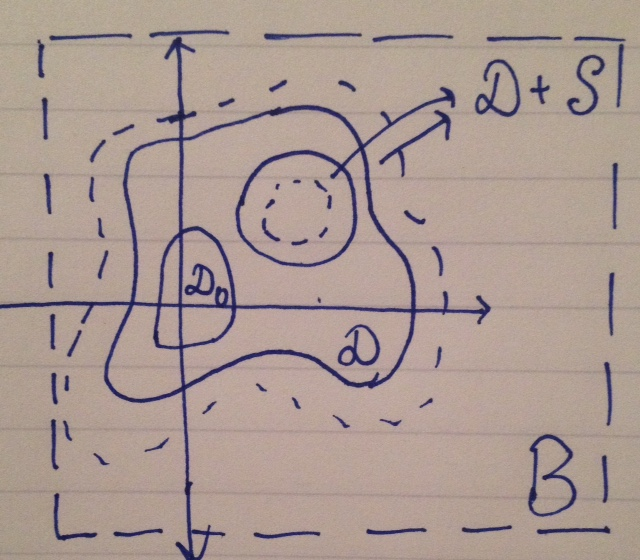
\includegraphics[scale = 0.5]{image5}
    \caption{Finite region enclosed in box $B$}
    \label{fig:finitebox}
\end{figure}

This immediately gives us the operator
\begin{align}
	E_k = 1 - \sum_{j=1}^{n_k} \ext{x_k^{a_k-j}}+\ext{x_k^{b_k+j}}\,,
\end{align}
which is equal to $E_k = 1$ when $n = 0$. Applying $E_1,\ldots, E_d$ sequentially ensures that we remove all monomials outside of $\mc D$. That is, $E = E_1\cdots E_d$. Since each of the operators is finite, their composition $\Gamma = LE$ is as well.
\end{proof}
\begin{theorem} Let $\mc D$ be a finite region in $\ze^d$ and $|\mc S| <\infty$. Then the operator $\Gamma = LE$ is of finite type.
\end{theorem}
\begin{proof} The region $\mc D$ lies within a bounding box $B$, so we may write $E = E' E''$, where $E' = E_1\cdots E_d$ from the lemma and $E''$ is the operator removing all monomials outside of $\mc D$ but inside the interior of $B$. $E''$ is finite since there are only finitely many points in that region. Since we are marking only finitely many points $\mc D_0 \subseteq \mc D$, $L$ is finite and finally, $\Gamma$ is finite.
\end{proof}

Also, we may handle semi-infinite regions if we are only marking finitely many points $\mc D_0$. The analysis is the same as above except that now one or more of $a_k, b_k$ may be infinite, and in this case we actually lose parts of $\Gamma_{B^c}$ and the operator is still finite.

\begin{definition} A random walk model with finitely many steps is of finite type if its extraction and marking operators $E$ and $L$ are of finite type, and its starting condition $q$ is of finite degree. Otherwise, we say the model is of infinite type.
\end{definition}
\begin{example} All the models so far has been of finite type, but not all models are of finite type. Consider a one-dimensional model on the whole line where we mark points $x_1^i$ with monomials $a_i$ using operator $L$. Then all equivalent marking operators $L'$ would have to have a term like $(a_i-1)\ext{x_1^i}$; otherwise, it would not act the same way on monomials in the model's reach $\ze$. Therefore, we must not have a finite operator $L'$ either.
\end{example}
Finite models are somewhat nice because they will have functional equations with finitely many terms and there is a chance that they will be amenable to the sort of analysis we have performed for quarter-plane walk models in the past. What follows is a rather easy application of the theory so far.

%=======================================
\section{Kernel Forms}
%=======================================
We can write out the functional equations in a way that highlights the kernel $K$ in the equation. We start out as follows
\begin{align}
	(1-tLES)Q &= 1\\
	(1-t(LE-1+1)S)Q &=1\\
	KQ + t(1-LE)SQ &= 1\,.
\end{align}
This is the form we see in the master functional equation. Another way we could have expanded is as follows
\begin{align}
\begin{split}
	(1-tLES)Q &= 1\\
	(1+LE(1-tS-1))Q &= 1\\
	LEKQ+(1-LE)Q &= 1\\
	LEKQ+(1-L)Q &= 1
\end{split}	
\end{align}
where $EQ = Q$ since $Q$ is already of a valid form. We can go with both ways at the same time as well.
\begin{align}\begin{split}
	KQ + t(1-LE)SQ &= 1\\
	KQ + (1-LE)(1-tS-1)Q &=1\\
	KQ + (1-LE)KQ - (1-L)Q &= 1\,.
\end{split}\end{align}
We can apply the inverse $L^{\um 1}$ to those equations too, in particular on the second one.
\begin{align}
\begin{split}
	L^{\um 1}(LEKQ+(1-LE)Q) &= 1
\end{split}	
\end{align}

The second form of the functional equation involving $L^{\um 1}$ should have less terms than the first one by virtue of separating $L$ and $E$ from one another. Using extraction operators, we can constrain random walks to lie within a finite region, semi-infinite strip, a semi-infinite sector or any other discrete shape (with diminishing returns for more complicated shapes, of course). Furthermore, using marking operators, we can easily track the behavior of random walks as they cross or interact with boundaries or interact with regions within. For example, we may consider walks interacting with the boundary of a box within some region in space. 

%=======================================
\section{Walks without interactions}
%=======================================
The Kernel forms above suggest an easier route for dealing with the models without interactions. Those models are equivalent to setting all the $a_k$'s to 1, and this is equivalent to removing all marking or unmarking operators. The first kernel form reduces to the simple functional equation
\begin{align}
	 E(KQ) = 1\,.
\end{align}
This suggests using the following substitution
\begin{align}
	Q = \frac{W}{x_{[d]} K}
\end{align}
so we have
\begin{align}
	x_{[d]} = x_{[d]}E(KQ) = x_{[d]}E\ol{x}_{[d]}W = \Gamma W\,,
\end{align}
where  $\Gamma = \Gamma_1\ldots\Gamma_d$ and 
\begin{align}
	\Gamma_k = x_kE_k\ol{x}_k = x_k(1-\ext{\ol{x}_k})\ol{x}_k = 1 - [x_k]^0\,.
\end{align}
Therefore, we have the functional equation for $W$ as
\begin{prop} Let $W = x_{[d]}KQ$, where $Q$ is the generating function for walks without interactions in the positive orthant
\begin{align}
	\Gamma W = \sum_{I\subseteq [d]}(-1)^{|I|} W_I^\oo= x_{[d]}\,.
\end{align}
\end{prop}
For example, in two dimensions we have
\begin{align}
	W(x_1,x_2) - W_1^0(x_2) -W_2^0(x_1) + W_{1,2}^{0,0} = x_1x_2\,.
\end{align}
Thus, we can write the solution to the problem as
\begin{align}
	Q = \frac{1}{x_{[d]}K}\left(x_{[d]}-\sum_{\emptyset \neq I\subseteq [d]}(-1)^{|I|} W_I^\oo\right)\,.
\end{align}
In two dimensions this becomes
\begin{align}
	Q(x_1,x_2) = \frac{x_1x_2+W_1^0(x_2)+W_2^0(x_1)-W_{1,2}^{0,0}}{x_1x_2(1-tS)}\,.
\end{align}
Of course, each $W_I^\oo$ depends on $Q_I^\oo$, so we could have seen this relationship from the master functional equation for $Q$ too.
Interestingly enough, this calculation points to a differential equation. Clearly, $W$ satisfies the differential equation
\begin{align}
	\del_1\del_2 W &= 1
\end{align}
\begin{prop} The function $Q$ for walks without interactions is D-finite in the $x_1,\ldots,x_d$ variables since it satisfies the inhomogeneous PDE
\begin{align}
	\del_1\ldots\del_d W = \del_1\ldots\del_d (x_1\ldots x_d KQ) = 1\,.
\end{align}
\end{prop}
We will see a more general relationship in a later chapter.

%=============================================

\begin{theorem} The generating function $Q$ for a random walk model of finite type is D-finite in the variables $\row xd$.
\end{theorem}
\begin{proof} We will use the kernel form for the functional equation
\begin{align}
	KQ + t(1- \Gamma)SQ = q.
\end{align}
Here $\Gamma' = 1- \Gamma$ is purely a coefficient extractor and it is of finite type, since $L$ and $E$ are finite. We will prove the theorem by finding the differential equation explicitly. Since the model is of finite type, we can bound the degree of $x_k$ that we see on either side of the functional equation. In one scheme we let $A_k$ be the largest power of $x_k$ that we need to clear a negative power of $x_k$ in $\Gamma'$ and in $q$. Then we let $B_k$ be the largest power of $x_k$ we see on either side. Once we multiply by $x_k^{A_k}$, we see that the degree of $x_k$ in the equation is $A_k+B_k$. We take the functional equation and multiply both sides by $x_{[d]}^{A}$. That is,
\begin{align}
	x_{[d]}^{A}(KQ + t\Gamma'SQ) = x_{[d]}^{A}q
\end{align}
and we attain a polynomial equation in the variables $\row xd$. We take the derivative operator
\begin{align}
	D = \del_{[d]}^{A+B+\one} = \del_1^{A_1+B_1+1}\ldots\del_d^{A_d+B_d+1}
\end{align}
and apply it to both sides of the equation to retrieve
\begin{align}
	D(x_{[d]}^{A}(KQ + t\Gamma'SQ)  = D(x_{[d]}KQ) = D(x_{[d]}^{A}q) = 0\,,
\end{align}
which follows since we are applying a larger number of derivatives than the degrees of the monomials and this clears all of them. The other scheme lets us obtain a potentially lower degree differential equation at the cost of homogeneity, if the degrees of $q$ are large. Let $A_k$ be the power of $x_k$ that we need to clear denominators on the left-hand side of the functional equation and $B_k$ be the largest power of $x_k$ on that side. Then we have $D$ as before, but this time it may have lower $A$ and $B$ values, since we are not taking $q$ into account. We have
\begin{align}
	D(x_{[d]}^{A}(KQ + t\Gamma'SQ)  = D(x_{[d]}KQ) = D(x_{[d]}^{A}q)\,.
\end{align}
\end{proof}
For example, let the powers of $x_k$ be $\{-3,-1,4\}$ and $\{-2,0,6\}$ on the left-hand side and right-hand side respectively. We see that $A_k = 3$ and $B_k = 6$. Then we are taking the $A_k + B_k + 1 = 10$-th derivative of both sides of the functional equation. In the second scheme we take $A_k = 3$ still, but $B_k = 4$ and we are taking the 8-th derivative with respect to $x_k$ this time. Even in the quarter-plane, we have models with non D-finite generating function (in the $t$ variable), but it turns out that every model so far considered is D-finite in the variables $\row xd$.

In order to solve the differential equation we need to investigate the kernel of the differential operator.
\begin{corollary}
The generating function $Q$ of a finite random model is given by
\begin{align}
	x_{[d]}^{A}KQ(x_1,\ldots,x_d;t) = \sum_{i=1}^d \sum_{j=0}^{B_i}Aij(x_1,\ldots,x_{i-1},x_i,\ldots, x_d,t) x_i^j\,,
\end{align}
where $A_{ij}$ are functions that need to be determined.
\end{corollary}
This kind of solution would have also appeared if we went through the calculations in the functional equation and extracted coefficients. However, this method is more efficient. If we had used the second scheme in the proof, we would have ended up with a slightly different form but maybe it would have had a slightly lower degree. It would involve an indefinite integral of $q$ and elements in the kernel of the differential operator.

%================================
\section{Examples of regions we can consider}
%================================

ZZPICTUREZZ

ZZPICTUREZZ

\begin{example}[Self-avoiding walks]

We can handle discrete self-avoiding random walks with this theory. If we pick a marking operator $\Gamma$ that marks every location on the plane, this will allow us to track the random walks' history. All we will need to do in the end is remove walks that have stepped at some location more than once. However, we will do this problem in a bit more detail as it serves as an example of the theory. To use the generating function iteration properly we need a sort of limiting argument. For the first $n$ steps we "only" require an operator covering the square region of $(2n+1)^2$ lattice points. The overall operator is defined through a limiting process of applying the full operator (or truncated version) on a finite Laurent polynomial. Let
\begin{align}
\Gamma_{i,j} = 1+b_{i,j}\ext{x_1^ix_2^j}
\end{align}
where as usual $b_{i,j} = a_{i,j}-1$. This operator takes a generating function and marks the monomial $x_1^ix_2^j$. We will be using a lot of these together, so we let
\begin{align}
\Gamma_n = \prod_{-n\leq i,j\leq n}\Gamma_{i,j}
\end{align}
To find a functional equation for SAWs on the plane we perform an iteration. Let $Q$ be the generating function for walks with history, that is, they have a mark for each coordinate they pass through, and let $Q^{\leq n}$ be the truncated version of this generating function. It is given by
\begin{align}
Q^{\leq n} = \sum_{k=0}^{n} Q_k t^k
\end{align}
where the initial condition is $Q_0 = a_{0,0}$. Starting from $Q_n$ we can find $Q_{n+1}$ by iterating with the step set $S$, marking with $\Gamma_{n+1}$ as follows
\begin{align}
	Q_{n+1} = \Gamma_{n+1}SQ_n
\end{align}
Using a computer we can easily iterate this to add more and more steps. We can also obtain $Q^{\leq n+1}$ from $Q^{\leq n}$ since
\begin{align}\begin{split}
	t\Gamma_{n+1}SQ^{\leq n} & = \sum_{k=0}^n \Gamma_{n+1}SQ_kt^{k+1}= \sum_{k=0}^n \Gamma_{k+1}SQ_kt^{k+1} = \sum_{k=0}^n Q_{k+1}t^{k+1} = Q^{\leq n+1}-Q_0
\end{split}\end{align}
or in other words
\begin{align}
	 Q^{\leq n+1} = a_{0,0} + t\Gamma_{n+1}SQ^{\leq n}
\end{align}
In the interest of finding a functional equation we would like to take the limiit of this as $n \to \infty$. For this we define $\Gamma$ to be the operator marking all monomials $x_1^ix_2^j$, acting in the following way
\begin{align}
	\Gamma x^i y^j = \Gamma_{\max(|i|,|j|)} x^i y^j
\end{align}
and extended by linearity. The limiting process is
\begin{align}
	Q = a_{0,0} + t \Gamma SQ
\end{align}
We finally have the functional equation for random walks with full history
\begin{align}
	(1 -t\Gamma S)Q = a_{0,0}.
\end{align}
As in the example of an infinte marking operator, it stands to reason that $\Gamma$ is of infinite type as well. From the equation we can retrieve the generating function $W$ for the SAWs by removing all walks with power of mark $a_{i,j}$ greater than 1. For this we need an operator that removes terms with more than one copy of a given label. Let
\begin{align}
	R_{i,j} &= \ext{a_{i,j}^0} + \ext{a_{i,j}}\\
	R_n &= \prod_{-n\leq i,j \leq n} R_{i,j}\\
	R &= \lim_{n\to \infty} R_n
\end{align}
where the limit is understood as in the example of $\Gamma$ above. The solution for $Q$ can also be restated as
\begin{align}
	Q = \sum_{k=0}^{\infty} t^k (\Gamma S)^{k}(a_{0,0}) = \sum_{k=0}^{\infty} t^k (\Gamma_k S)^{k}(a_{0,0}) 
\end{align}
We can either redo the analysis, applying $R$ at every iteration, or we can apply $R$ to $Q$ and find
\begin{align}
	W = RQ = \sum_{k=0}^{\infty} t^k R(\Gamma S)^{k}(a_{0,0}) = \sum_{k=0}^{\infty} t^k (R\Gamma S)^{k}(a_{0,0}) 
\end{align}
We can write this as a functional equation
\begin{align}
	\mc{L} W = (1-t\Sigma)W = (1-tR\Gamma S)W = a_{0,0}.
\end{align}
It is not clear if the operator $R\Gamma$ is of finite type. Now it is enough to set all the remaining labels to 1 and we will find the full generating function of SAWs with steps from $\mc{S}$.

The discussion lends itself nicely to generalization where we have $d$ variables and operators $\Gamma_{i_1,\ldots,l_d}$, $R_{i_1,\ldots,i_d}$, and so on, defined analogously. The eigenpair discussion works out in the same way with eigenfunctions for $\lambda = 1$
\begin{align}
	u = \frac{a_{i_1,\ldots,i_d}^2 a_{j_1,\ldots,j_d}^m}{a_{k_1,\ldots,k_d}S}x_1^{r_1}\ldots x_d^{r_d} t^n
\end{align}
Also, we can constrain the SAWs on a part of $\ze^d$ with an extraction operator $E$ and mark special locations with an operator $L$. The functional equation is
\begin{align}
	(1- tLE\Sigma)W = a_{0,\ldots,0}
\end{align}
for arbitrary number of dimensions, with regional constraints and marking of special locations.
\end{example}

\endinput

%================================================================
%================================================================
%================================================================
%================================================================
%================================================================

%================================
\section{Coefficient Extraction Equations}
%================================

The work so far is strongly hinting towards a theory of ordinary and partial coefficient extraction equations - OCEs and PCEs. Here we will work out some of the theory. We start with a partial coefficient extraction operator of finite type
\begin{definition}$\mc{L}$ is a coefficient operator if
\begin{align}
	\mc{L} = \sum_{\substack{I\subseteq [d]\\ J \subseteq \ze^d}}a_{I,J}[x_I^J] = K + \mc{E}
\end{align}
where $K$ is the kernel of the operator, $\mc{E}$ is the pure extraction part
\begin{align}
	\mc{E}  = \sum_{\substack{I\subseteq [d],I\neq \emptyset\\ J \subseteq \ze^d}}a_{I,J}[x_I^J]
\end{align}
and all the coefficients are Laurent polynomials in the $x$ variables and perhaps some other variables. The operator is ordinary if $d = 1$ and partial if $d \ge 2$. The operator is either of monomial type where the coefficients are monomials or of polynomial type if one or more coefficients is a Laurent polynomial in $x_1,\ldots,x_d$.
\end{definition}
\begin{definition} An ordinary/partial coefficient equation (OCE/PCE) is one of the form $\mc{L} Q = q$ for some functions $Q$ and $q$ where $\mc{L}$ is an ordinary/partial coefficient operator. The equation is homogeneous if $q = 0$ and inhomogeneous if $q \neq 0$.
\end{definition}
The question is whether we can solve these kinds of equations in general, and what their solutions may look like. In the previous section we found that if $\mc{L}$ is finite then the function $Q$ is D-finite in the $x$ variables while it may not necessarily be D-finite in the $t$ variable or any other variable (parameter) that appears in the coefficients.

\begin{example} The operator $\Gamma$ in this section is a partial coefficient operator with monomial coefficients.
\end{example}

\begin{example} We can transform the functional equation for a finite random walk model into a PCE. To do so, we note that $K$ is the same in both forms. The part requiring some work is the one that has to do with the term $(1-\Gamma)SQ$ which is a pure extraction of $SQ$. We can expand $S$ into its monomials. Then $(1-\Gamma)S$ fully expands into monomials of the form
\begin{align}
	a_{I,J}\ext{x_I^J}x_A^B
\end{align}
we can pull terms inside $[x_I^J]$ from the right. In the end the $S$ is absorbed within the operator and istead of having monomial coefficients it now has polynomial coefficients. It may be useful to write an operator $\mc{L}$ in the form
\begin{align}
	\mc{L} = K + \Gamma'S
\end{align}
for some monomial operator $\Gamma'$.
\end{example}

%================================
\section{Connection with Fredholm Theory}
%================================
Suppose that we are given the equation in the form
\begin{align}
	KQ +t\Gamma'SQ = q
\end{align}
where
\begin{align}
	\Gamma' = \sum_{I,J}a_{I,J} x_I^J[x_I^J]
\end{align}
where we only have finite-sized $J$'s and $\emptyset \neq I\subseteq [d]$. From complex analysis we know that for a function $f(x)$ given by a power series and for $x$ within the region of convergence
\begin{align}
	[x^n]f(x) = f_n = \frac{1}{2\pi i}\int_\gamma \frac{f(z)}{z^{n+1}}dz
\end{align}
and
\begin{align}
	f(x) = \frac{1}{2\pi i}\int_\gamma \frac{f(z)}{z-x}dz
\end{align}
where in the first case $\gamma$ winds CCW around the origin within the region of convergence and in the second case $\gamma$ winds around $x$ within the region of convergence. The idea is to combine these two expressions for many dimensions (at least formally) to represent the operator $\mc{L}$ in integral form. We have for $|I| = n$
\begin{align}
	[x_I^J]f(x_1,\ldots,x_d)= \frac{1}{(2\pi i)^{n}}\int\cdots\int_\gamma \frac{f}{z_I^{J+1}}dz_I
\end{align}
where $f$ has $x_i = z_i$ for $i \in I$ and the rest are still $x$'s. If we use this representation we will have different numbers of iterations of the integral for different coefficient. We might as well go all-out and write
\begin{align}
	[x_I^J]f(x_1,\ldots,x_d)= \frac{1}{(2\pi i)^d}\int\cdots\int_\gamma \frac{f}{z_I^{J+1}(z-x)_{I^c}}dz_{[d]}
\end{align}
where now $x_i = z_i$ in $f$ and 
\begin{align}
	(z-x)_P = \prod_{p\in P} (z_p-x_p)
\end{align}
This allows us to write The operator like this
\begin{align}
	(K+t\Gamma'S)Q&= \frac{1}{(2\pi i)^d}\int\cdots\int_\gamma \left(\frac{K}{(z-x)_{[d]}} +t S\sum_{I,J}\frac{a_{I,J}}{z_I^{J+1}(z-x)_{I^c}}\right)Q dz_{[d]}\\
	& = \frac{1}{(2\pi i)^d}\int\cdots\int_\gamma \frac{1}{(z-x)_{[d]}}\left(K +t S\sum_{I,J}\frac{a_{I,J}(z-x)_I}{z_I^{J+1}}\right)Q dz_{[d]}\\
	&= \frac{1}{(2\pi i)^d}\int\cdots\int_\gamma R_0Q dz_{[d]}
\end{align}
Now to turn this into a $d$-dimensional Fredholm problem we will need to parametrize the integral. One way that might work is to set $z_k = r_k \exp(i\theta_k)$ and $x_k = s_k e^{i\phi_k}$. Since $dz_k = r_k i e^{i\theta_k}$, we have
\begin{align}
(K+t\Gamma'S)Q = \frac{r_{[d]}}{(2\pi)^d}\int_0^{2\pi}\cdots\int_0^{2\pi} e^{i\theta_1}\ldots e^{i\theta_d}R_0Q d\theta_{[d]} = q(\phi_1,\ldots,\phi_d)\,,
\end{align}
so if we write
\begin{align}
R = \exp(i(\theta_1+\ldots + \theta_d))R_0(\phi_1,\ldots,\phi_d,\theta_1,\ldots,\theta_d)
\end{align}
we have the inhomogeneous Fredholm equation of the first kind in $d$ dimensions
\begin{align}
	\int_0^{2\pi}\cdots\int_0^{2\pi} RQ d\theta_1\ldots d\theta_d= g
\end{align}
where $R$ is the kernel and $g = (2\pi)^dq/r_{[d]}$ and $Q$ is in terms of $\theta_k$'s. Perhaps Fredholm theory can be applied in solving the random walk models in man dimensions. Perhaps this will also lead to a good inner product on the space where $Q$ lives.

%================================
\section{Reformulations of Problems}
%================================

\subsection{Using marking operators instead of extraction operators}
An initially promising idea is to use a marking operator instead of an extraction operator with the goal of removing those marked walks at a later stage. The added benefit is that we would be working with invertible operators throughout the majority of the analysis. The downside is that now the walks will not be constrained and $Q$ will no longer be a power series in the $x$ variables. We may get further problems. Instead of $E = 1- \ext{\ol{x}}$ we take $\tilde E = 1 + (a_{\um 1}-1)\ext{x}$ with the idea that if we set $a_{\um 1} = 0$ we will obtain $E$. To this end the functional equation is
\begin{align}
	(1-tL\tilde E S)\tilde Q = 1
\end{align}
which after inversion turns into
\begin{align}
	(\tilde E^{\um 1} L^{\um 1} -tS) \tilde Q = \tilde E^{\um 1} L^{\um 1} 1 = \alpha
\end{align}
One benefit of this is that we do not have a mixing between the $E$, $L$ operators and $S$. The downside is we have more $Q$ extractions on their own. We can write this in kernel form as
\begin{align}
	K \tilde Q = \alpha + (1 - L^{\um 1}\tilde E^{\um 1}) \tilde Q
\end{align}
where the operator $1- L^{\um 1}\tilde E^{\um 1}$ is composed entirely of coefficient extractions.
\subsection{Considering a symmetrical super-problem}
An extension of the previous idea is to symmetrize the problem by also marking parts on the other side of the origin. Instead of just marking walks on the axes and on lines where one coordinate is $-1$ we can also mark walks on lines with one coordinate $+1$. This leads to a symmetrical arrangement of marking operations on both sides of the origin. We have the equation
\begin{align}
	(1- tLS)\tilde Q = (1- t L_{\um 1}L_0L_1 S)\tilde Q = 1
\end{align}
We can skip the marking of the axes with $L_0$ if we do not wish to investigate wall interactions. In general, we may mark more locations in space so we can combine all of these operators into one called $L$. Then we have
\begin{align}
	(1- tLS)\tilde Q = 1
\end{align}
or in kernel forms
\begin{align}
	K\tilde Q = L^{\um 1}(1) + (1- L^{\um 1})\tilde Q
\end{align}

\endinput
\begin{example} Here is an example that may hint at the flavour of the OCE/PCE problems. Suppose we start with the fibonacci recurrence relation
\begin{align}
F_{n+2} =F_{n+1}+F_n
\end{align}
with some initial conditions for $f_0$ and $f_1$. We can perform the standard generating function solution approach via summing all equations. Let
\begin{align}
	F(x) = \sum_{n=0}^\infty F_n x^n
\end{align}
be the generating function for the fibonacci-like numbers. Note that $[x^n] F(x) = F_n$. We have
\begin{align}
	F_{n+2} &= F_{n+1}+F_n\\
	F_{n+2} x^{n+2}&= F_{n+1}x^{n+2}+F_nx^{n+2}\\
	\sum_{n=0}^{\infty} F_{n+2} x^{n+2}&= x\sum_{n=0}^{\infty}F_{n+1}x^{n+1}+x^2\sum_{n=0}^{\infty}F_nx^n\\
	F - F_1 x - F_0 &= x (F-F_0) + x^2 F
\end{align}
Pulling like terms together and putting everything on one side gives
\begin{align}
	(1-x - x^2) F - x F_1 + (x-1) F_0 = 0
\end{align}
This is a homogeneous OCE with ordinary coefficient operator$\mc{L}$ (Fibonacci operator?) with kernel $K = 1 - x - x^2$ and polynomial coefficients
\begin{align}
	\mc{L} = (1-x-x^2) + (x-1)[x^0]-x[x] = K + \mc{E}
\end{align}
The typical solution to the problem specifies initial conditions $F_0$ and $F_1$ and solves the problem as
\begin{align}
	F(x) = \frac{(x-1)F_0-x F_1}{1-x-x^2} = \frac{{\mc{E}}(F)}{K}
\end{align}
That is, it relies on the initial condition for $\mc{E}$ in order to solve the equation. We also see that if we do not specify the initial conditions we do not get a unique solution. In the random walks models we have unique solutions because of the iterative nature of the problems. With these points in mind we may try the vanishing kernel method by supplying a root of $K$ namely $x = \sigma$. These roots are
\begin{align}
\sigma_1 = -\varphi, \sigma_2 = \ol{\varphi}
\end{align}
where $\varphi$ is the golden ratio. Then plugging either one of these into the OCE leads to
\begin{align}
(\sigma-1)F_0 = \sigma F_1
\end{align}
\begin{align}
	 F_1 &= (1-\ol{\sigma}_1)F_0 = \varphi F_0\\
	 \text{ or } F_1 &=(1-\ol{\sigma}_2)F_0 = -\ol{\varphi} F_0
\end{align}
That is, if we want the vanishing kernel method to work we must have that $F_1$ is related to $F_0$ directly via the golden ratio. By induction we can show that $F_n = \varphi^n F_0$ in the first case and $F_n = (-\ol{\varphi})^n F_0$ in the second case.

What about the persistent kernel method? We want to apply a transformation $y = y(x)$ to $K$ that leaves it the same. That is,
\begin{align}
	K(y) = 1 - y - y^2 = K(x) = 1 - x - x^2
\end{align}
Collecting terms on one side yields
\begin{align}
	(y-x)(1+x+y) = 0
\end{align}
That is, the group $G$ that preserves the kernel is composed of the identity transformation and the the transformation $g(x) = -x-1$. We want a $F(-1-x)$ to converge which may not necessarily be true. Instead we multiply the whole functional equation by $\ol{x}$ to find
\begin{align}
\ol{x} \mc{L} = (\ol{x}-1-x) + (1-\ol{x})[x^0]-[x^1]
\end{align}
This new kernel $K$ is nicer. We have
\begin{align}
	K = \ol{x}-1-x = \ol{y}-1-y
\end{align}
rearranging this equality gives
\begin{align}
	(y-x)(1+\ol{x}\ol{y}) = 0
\end{align}
and thus, the group $G$ is generated by the identity transformation and $g(x) = -\ol{x}$ which is of order 2, so $|G| = 2$. We have the two equation
\begin{align}
KF +(1-\ol{x})F_0 - F_1 &= 0\\
KgF + (1+x)F_0  - F_1 &=0
\end{align}
Furthermore, emulating the orbit method, we have
\begin{align}
	(1-g)xKF = K(xF+\ol{x}gF)  = (x+\ol{x})(F_1-F_0)
\end{align}
If $F_1 \neq F_0$ we can write
\begin{align}
	xF+\ol{x}gF &= \frac{(x+\ol{x})}{K}(F_1-F_0) \\
	&= \frac{1+x^2}{1-x-x^2}(F_1-F_0) \\
	&= (1+x+3x^2+O(x^3))(F_1-F_0)
\end{align}
Extracting the $[x]$ coefficient yields
\begin{align}
	F_0 +[x^2]F(-\ol{x}) = F_0 = F_1 - F_0
\end{align}
so $F_1= 2 F_0$ and we find
\begin{align}
	xF+\ol{x}F(-\ol{x}) = F_0 \frac{1+x^2}{1-x-x^2}
\end{align}
Taking the positive part of this yields
\begin{align}
	xF= F_0 \frac{1+x^2}{1-x-x^2}
\end{align}
\end{example}
I think there is something wrong with the example but that is just me. We can demonstrate the D-finiteness by taking the second derivative of $xKF$
\begin{align}
	\del_x^2((1-x - x^2) F - x F_1 + (x-1) F_0) = \del_x^2(xKF) = 0
\end{align}

%================================
\subsection{Eigenpairs}
%================================
We can try finding eigenvalues and eigenfunctions of $\mc{L}$. Let $\mc{L}u = \lambda u$. Writing it out leaves us with
\begin{align}
	t\Sigma u = (1-\lambda)u
\end{align}
So if $\lambda = 1$, $u\in \ker(\Sigma)$. That is, $R\Gamma S u = 0$. In other words, $\Gamma S u$ only has terms that involve powers greater than 1 of $a_{i,j}$ for various $i,j$. Suppose that
\begin{align}
	\Gamma S u = a_{i,j}^2 f(x_1,x_2)
\end{align}
Then
\begin{align}
	u  = \frac{a_{i,j}^2}{S}\Gamma^{\um 1}(f)
\end{align}
So we here we can let
\begin{align}
		f = a_{k,l}^m x_1^rx_2^s t^n
\end{align}
and we find that
\begin{align}
	u =  \frac{a_{i,j}^2 a_{k,l}^m}{a_{r,s}S}x_1^r x_2^s t^n
\end{align}
Thus, the kernel of $\Sigma$ is generated by these functions for all coefficients $i,j,k,l,r,s,n \in \ze$ and $m\ge 0$. This may perhaps prove useful later on. Now, if we look at eigenvalues $\lambda \neq 1$ we have to solve the equation
\begin{align}
	t \Sigma u = (1-\lambda) u
\end{align}
Because of the $t$, if $u$ is a finite order laurent series in $t$ with first nonzero coeficient $u_n$. We find that since $\Sigma$ does not interact with the $t$ monomials
\begin{align}
	\Sigma u_n = \mu u_{n-1} = 0
\end{align}
and this forces all $u_k$ coefficients to be zero. Therefore, $\Sigma$ has no other eigenvalues except 1 among the finite order power series in $t$.